
\chapter{Results}
\section{Hardware and Metrics}
The hardware used for the experiments is :\begin{itemize}
  \item Intel Xeon CPU W3550 @3.07 GHz with 8GB RAM and four cores
  \item NVIDIA GeForce GTX680 (which was analytically discussed in Chapter 2)
\end{itemize}Time was measured using clock() function and is presented in seconds.
All experiments were performed with full optimizations turned on.CPU code was compiled with Intel's compiler (icc) and GPU code with nvcc.
\section{Experiments}
The performance results for each implementation, described in Chapter 4, are presented in the following tables . The execution time is the average of ten measurements for each case. Furthermore, the speed - up between CPU and GPU is given.

The correctness of results was validated with relative MATLAB functions. The results of the CPU have been identified with the results of the GPU.
\newpage
\subsection{Single Precision Performance}


  

\begin{table}[H]
\caption{Cyclic Reduction (first version) execution time (SP)} 
\centering 
\begin{tabular}{| l | p{3cm} | p{3cm} |} 
\hline\hline 
Size & CPU & GPU  \\ [0.8ex] 
\hline 
$2^{21}$ & $0.113$ & $0.02$\\ 
$2^{22}$ & $0.216$ & $0.034$\\
$2^{23}$ & $0.455$ & $0.063$\\
$2^{24}$ & $0.909$ & $0.126$\\
$2^{25}$ & $1.82$ & $0.25$ \\ 
$2^{26}$ & $3.65$ & $0.50$ \\[1ex] 
\hline 
\end{tabular}
\label{table:cr_first} 
\end{table}

\begin{figure}[H]
   \centering
       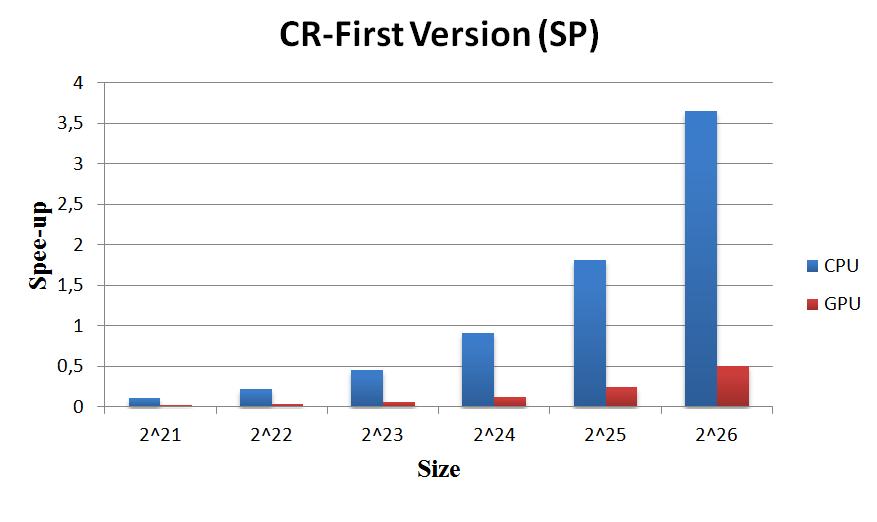
\includegraphics[width=1\textwidth]{grafhmata/cr_first_sp.png}
   \caption{CPU-GPU Cyclic Reduction(SP)}
   \label{fig:CPU-GPU Cyclic Reduction(SP)}
\end{figure}

\begin{table}[H]
\caption{Cyclic Reduction (first version) speed - up (SP)} 
\centering 
\begin{tabular}{| l | p{3cm} |} 
\hline\hline 
size	 & Speed - up  \\  [0.8ex] 
\hline        
        $2^{21}$ & $5.38$      \\ 	
        $2^{22}$ & $6.35$     \\ 	
        $2^{23}$ & $7.22$      \\ 
        $2^{24}$ & $7.21$    \\ 
        $2^{25}$ & $7.28$     \\ 
        $2^{26}$ & $7.1$       \\ [1ex] 
        \hline
\end{tabular}
\label{table:cr_first_spup} 
\end{table}

\begin{figure}[H]
   \centering
       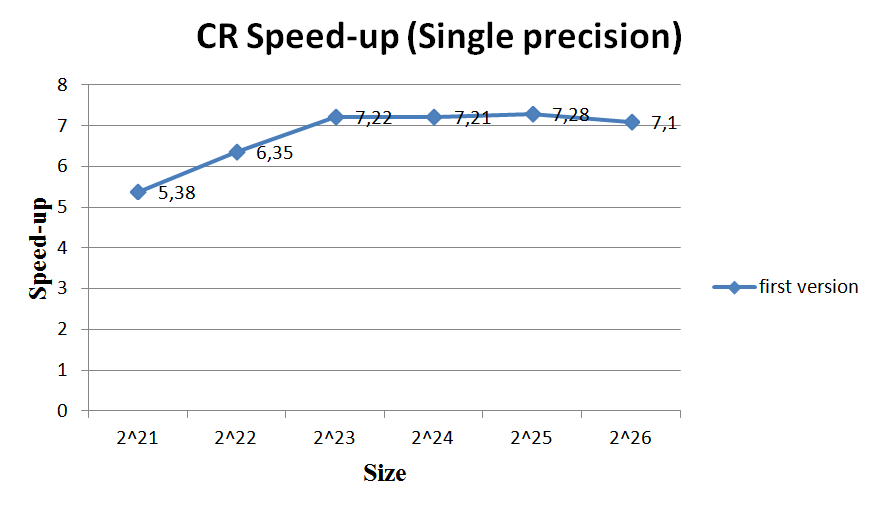
\includegraphics[width=1\textwidth]{grafhmata/cr_first_sp_speedup.png}
   \caption{Speedup Cyclic Reduction(SP)}
   \label{fig:Speedup Cyclic Reduction(SP)}
\end{figure}

As can be observed from the above table the speed-up increases as the data set increases.
This is normal because GPU performs better when has more data to process. It is worth mentioning
that a decrease is observed from size = $2^25$ to size = $2^26$. To be explained that measurements were made in relation to computation to memory transfers ratio. It was observed that from a certain size memory transferring 
consumes more time than the actual computation.

\begin{table}[H]
\caption{Cyclic Reduction (padding version) execution time (SP)} 
\centering 
\begin{tabular}{| l | p{3cm} | p{3cm} |} 
\hline\hline 
Size & CPU & GPU  \\ [0.8ex] 
\hline 
$2^{21}$ & $0.108$ & $0.021$\\ 
$2^{22}$ & $0.214$ & $0.035$\\
$2^{23}$ & $0.456$ & $0.066$\\
$2^{24}$ & $0.877$ & $0.115$\\
$2^{25}$ & $1.769$ & $0.251$ \\ 
$2^{26}$ & $3.546$ & $0.509$ \\[1ex] 
\hline 
\end{tabular}
\label{table:cr_padding} 
\end{table}



\begin{table}[H]
\caption{Cyclic Reduction (padding version) speed - up (SP)} 
\centering 
\begin{tabular}{| l | p{3cm} |} 
\hline\hline 
size	 & Speed - up  \\  [0.8ex] 
\hline        
        $2^{21}$ & $4.14$      \\ 	
        $2^{22}$ & $6.11$     \\ 	
        $2^{23}$ & $6.90$      \\ 
        $2^{24}$ & $7.62$    \\ 
        $2^{25}$ & $7.04$     \\ 
        $2^{26}$ & $6.96$       \\ [1ex] 
        \hline
\end{tabular}
\label{table:cr_padding_spup} 
\end{table}

The padding technique did not increase the performance of the implementation. That happened because  there was no significant divergence in the code.


In the following tables it is presented the speed up of the Buneman algorithm for different geometries, where Q is the size of block and N the number of blocks. In the first six tables, the size of block remains stable while the number of blocks is increasing. As GPU(first) is mentioned the first implementation and as GPU(second) the one with the sliding window optimization. GPU results were compared with sequential CPU and multithreaded (4 threads) CPU.  

\newpage
    \begin{table}[H]
\caption{Block Cyclic Reduction N=3} 
\centering 
\begin{tabular}{| l |  p{1cm} |p{2,5cm}| p{2,5cm} |  p{2,5cm}| p{2,5cm}  |} 
\hline\hline 
N & Q & CPU(parallel) & CPU(seq) & GPU(first)  & GPU(second) \\ [0.8ex] 
\hline 
$3$ &	$127$ & $0.000$	& $0.000$ & $0.005$ &  $0.004$ \\
$3$ &	$255$ & $0.005$	&	$0.000$ & $0.020$ & $0.020$ \\
$3$ &	$511$ & $0.027$	&	$0.060$ & $0.062$ & $0.062$ \\
$3$ &	$1023$ & $0.168$	&	$0.450$ & $0.145$ & $0.147$ \\
$3$ &	$2047$ & $1.058$	&	$3.160$ & $0.403$ & $0.403$ \\
$3$ &	$4095$ & $7.392$	&	$23.940$ & $1.400$ & $1.398$ \\[1ex]
\hline 
\end{tabular}
\label{table:bcr_n=3} 
\end{table}

\begin{table}[H]
\caption{Block Cyclic Reduction N=7} 
\centering 
\begin{tabular}{| l |  p{1cm} |p{2,5cm}| p{2,5cm} |  p{2,5cm}| p{2,5cm}  |} 
\hline\hline 
N & Q & CPU(parallel) & CPU(seq) & GPU(first)  & GPU(second)\\ [0.8ex] 
\hline
$7$ &	$127$ & $0.002$	&	$0.000$ & $0.010$ & $0.007$ \\
$7$ &	$255$ & $0.015$	&	$0.020$ & $0.043$ & $0.040$ \\
$7$ &	$511$ & $0.075$	&	$0.170$ & $0.170$ & $0.168$ \\
$7$ &	$1023$ & $0.495$	&	$1.280$ & $0.390$ & $0.385$ \\
$7$ &	$2047$ & $3.030$	&	$9.260$ & $1.050$ & $1.085$ \\
$7$ &	$4095$ & $22.965$	&	$70.540$ & $3.795$ & $3.763$ \\[1ex]
\hline 
\end{tabular}
\label{table:bcr_n=7} 
\end{table}

   \begin{table}[H]
\caption{Block Cyclic Reduction N=15} 
\centering 
\begin{tabular}{| l |  p{1cm} |p{2,5cm}| p{2,5cm} |  p{2,5cm}| p{2,5cm}  |} 
\hline\hline 
N & Q & CPU(parallel) & CPU(seq) & GPU(first)  & GPU(second) \\ [0.8ex] 
\hline
$15$ &	$127$ & $0.007$	&	$0.010$ & $0.020$ & $0.018$ \\
$15$ &	$255$ & $0.035$	&	$0.060$ & $0.087$ & $0.085$ \\
$15$ &	$511$ & $0.175$	&	$0.410$ & $0.385$ & $0.390$ \\
$15$ &	$1023$ & $1.175$	& $3.080$  & $0.905$ & $0.892$ \\
$15$ &	$2047$ & $7.698$	&	$22.800$ & $2.432$ & $2.425$ \\
$15$ &  $4095$ & $53.650$	&	$174.750$ & $8.623$ &  $8.590$ \\[1ex]
\hline 
\end{tabular}
\label{table:bcr_n=15} 
\end{table}

   \begin{table}[H]
\caption{Block Cyclic Reduction N=31} 
\centering 
\begin{tabular}{| l |  p{1cm} |p{2,5cm}| p{2,5cm} |  p{2,5cm}| p{2,5cm} |} 
\hline\hline 
N & Q & CPU(parallel) & CPU(seq) & GPU(first)  & GPU(second) \\ [0.8ex] 
\hline
$31$ &	$127$ & $0.018$	&	$0.020$ & $0.038$ & $0.038$ \\
$31$ &	$255$ &	$0.070$	& $0.130$ & $0.185$ & $0.190$ \\
$31$ &	$511$ &	$0.365$	& $0.920$ & $0.827$ & $0.820$ \\
$31$ &	$1023$ &	$2.392$	& $6.870$ & $1.913$ & $1.910$ \\
$31$ &	$2047$ & $17.355$	&	$51.290$  & $5.215$ & $5.215$ \\
$31$ &	$4095$ & $117.445$	&	$394.260$ & $18.135$ & $18.083$ \\ [1ex]
\hline 
\end{tabular}
\label{table:bcr_n=31} 
\end{table}

   \begin{table}[H]
\caption{Block Cyclic Reduction N=63} 
\centering 
\begin{tabular}{| l |  p{1cm} |p{2,5cm}| p{2,5cm} |  p{2,5cm}| p{2,5cm} |} 
\hline\hline 
N & Q & CPU(parallel) & CPU(seq) & GPU(first)  & GPU(second) \\ [0.8ex] 
\hline

$63$ &	$127$ & $0.040$	&	$0.050$ & $0.075$ & $0.072$ \\
$63$ &	$255$ & $0.153$	&	$0.280$ & $0.363$ & $0.377$\\
$63$ &	$511$ & $0.745$	&	$1.940$ & $1.690$ & $1.685$ \\
$63$ &	$1023$ & $5.017$	&	 $14.660$ & $3.973$ & $3.983$ \\
$63$ &	$2047$ & $34.463$	&	$109.570$ & $10.705$ & $10.690$ \\
$63$ &	$4095$ & $249.585$	&	$844.420$ & $36.375$ & $36.393$ \\[1ex]
\hline 
\end{tabular}
\label{table:bcr_n=63} 
\end{table}

   \begin{table}[H]
\caption{Block Cyclic Reduction N=127} 
\centering 
\begin{tabular}{| l |  p{1cm} |p{2,5cm}| p{2,5cm} |  p{2,5cm}| p{2,5cm} |} 
\hline\hline 
N & Q & CPU(parallel) & CPU(seq) & GPU(first)  & GPU(second) \\ [0.8ex] 
\hline
$127$ &	$255$ & $0.298$	&	$0.580$ &	$0.757$ & $0.750$ \\
$127$ &	$511$ & $1.530$	&	$4.000$ & 	$3.420$ & $3.425$ \\
$127$ &	$1023$ & $10.340$	& $30.280$ & 	$7.925$ & $8.038$ \\
$127$ &	$2047$ & $71.278$	& $227.610$ & 	$21.520$ & $21.497$ \\
$127$ &	$4095$ & $514.878$	& $1753.420$ & 	$72.642$ & $72.588$\\[1ex]
\hline 
\end{tabular}
\label{table:bcr_n=127} 
\end{table}


\begin{figure}[H]
   \centering
       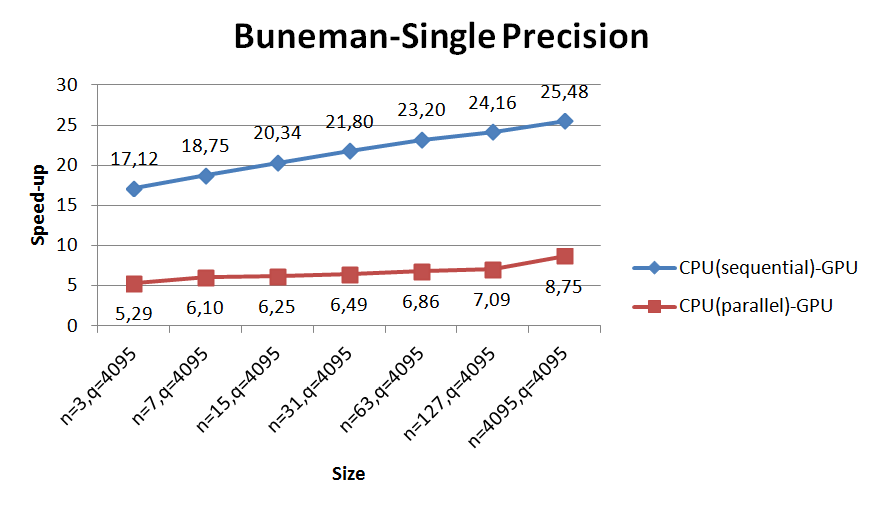
\includegraphics[width=1\textwidth]{grafhmata/buneman_sp_speedup.png}
   \caption{Speedup Buneman(SP)}
   \label{fig:Speedup Buneman(SP)}
\end{figure}


   \begin{table}[H]
\caption{Block Cyclic Reduction N=Q} 
\centering 
\begin{tabular}{| l |  p{1cm} |p{2,5cm}| p{2,5cm} |  p{2,5cm}| p{2,5cm} | } 
\hline\hline 
N & Q & CPU(parallel) & CPU(seq) & GPU(first)  & GPU(second) \\ [0.8ex] 
\hline
$127$ &	$127$ & $0.078$	&	$0.100$ & $0.147$ & $0.150$ \\
$255$ &	$255$ & $0.915$	&	$1.200$ & $1.487$ & $1.525$ \\
$511$ &	$511$ & $10.177$	&	$16.470$ & $13.797$ & $13.778$ \\
$1023$ &	$1023$ & $84.858$	&	$252.080$ & $63.520$ & $63.470$ \\
$2047$ &	$2047$ & $1175.078$	&	$3802.470$ & $331.875$ & $331.758$ \\
$4095$ & $4095$  & $20203.910$	&  $58816.617$ & $--$ & $2308.483$ \\[1ex]
\hline 
\end{tabular}
\label{table:bcr_n=q} 
\end{table} 

\begin{figure}[H]
   \centering
       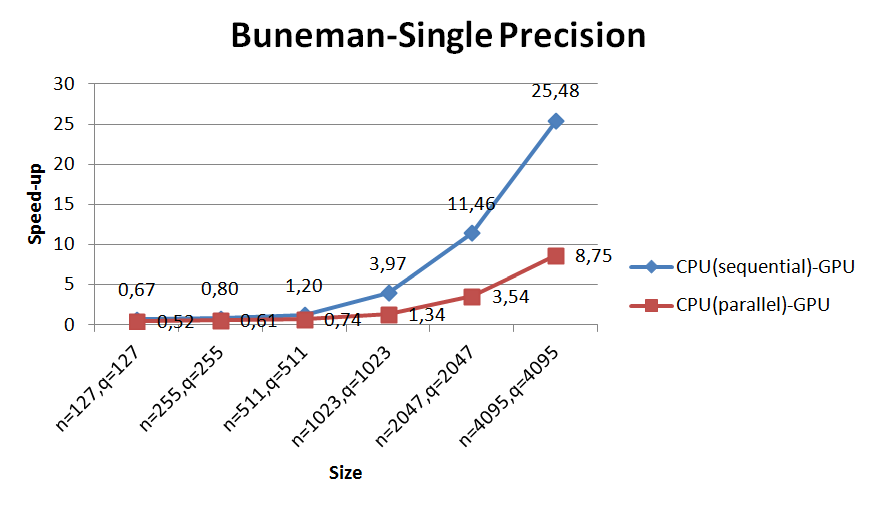
\includegraphics[width=1\textwidth]{grafhmata/buneman_sp_speedup_nq.png}
   \caption{Speedup Buneman N=Q (SP)}
   \label{fig:Speedup Buneman N=Q (SP)}
\end{figure}

As can be observed a remarkable speed -up up to 25x can be achieved using GPU instead of sequential CPU.
It is worth to be mentioned that as the size increases the speed - up increases but the rate of this growth
decreases.The maximum speed-up is achieved when we use the maximum Q size. This is normal because the GPU work load depends on Q size since concerns the inner loop which actually runs on GPU.

\subsection{Double Precision Performance}


\begin{table}[H]
\caption{Cyclic Reduction (first version) execution time (DP)} 
\centering 
\begin{tabular}{| l | p{3cm} | p{3cm} |} 
\hline\hline 
Size & CPU & GPU  \\ [0.8ex] 
\hline 
        $2^{21}$ & $0.148$& $0.033$ \\ 	
        $2^{22}$ & $0.314$& $0.06$  \\ 	
        $2^{23}$ & $0.619$& $0.119$ \\ 
        $2^{24}$ & $1.213$& $0.236$ \\ 
        $2^{25}$ & $2.33$& $0.47$  \\ 
        $2^{26}$ & $--$& $--$      \\ [1ex]
\hline 
\end{tabular}
\label{table:cr_first_double} 
\end{table}

\begin{figure}[H]
   \centering
       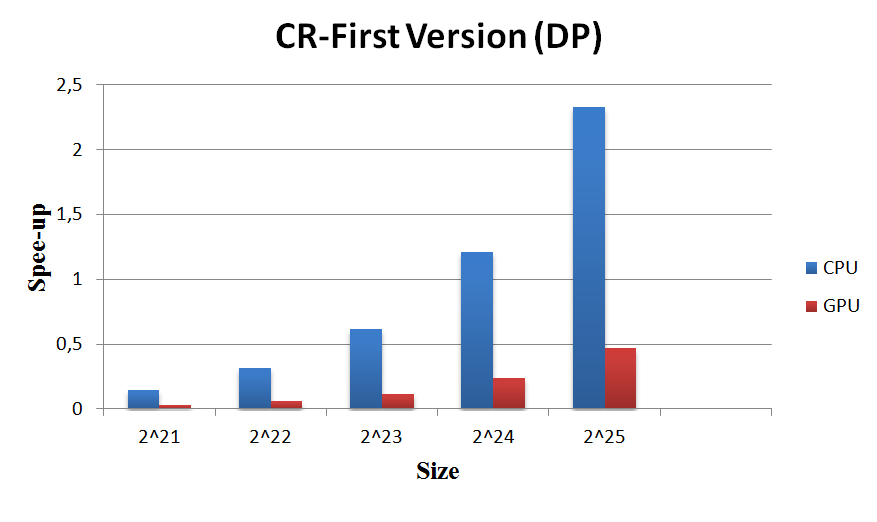
\includegraphics[width=1\textwidth]{grafhmata/cr_first_dp.png}
   \caption{CPU-GPU Cyclic Reduction(DP)}
   \label{fig:CPU-GPU Cyclic Reduction(DP)}
\end{figure}

\begin{table}[H]
\caption{Cyclic Reduction (first version) speed - up (DP)} 
\centering 
\begin{tabular}{| l | p{3cm} |} 
\hline\hline 
size	 & Speed - up  \\  [0.8ex] 
\hline        
        $2^{21}$ & $4.48$      \\	
        $2^{22}$ & $5.23$     \\
        $2^{23}$ & $5.2$      \\ 
        $2^{24}$ & $5.13$    \\ 
        $2^{25}$ & $4.95$     \\ 
        $2^{26}$ & $--$       \\ [1ex]
        \hline
\end{tabular}
\label{table:cr_first_double_spup} 
\end{table}

\begin{figure}[H]
   \centering
       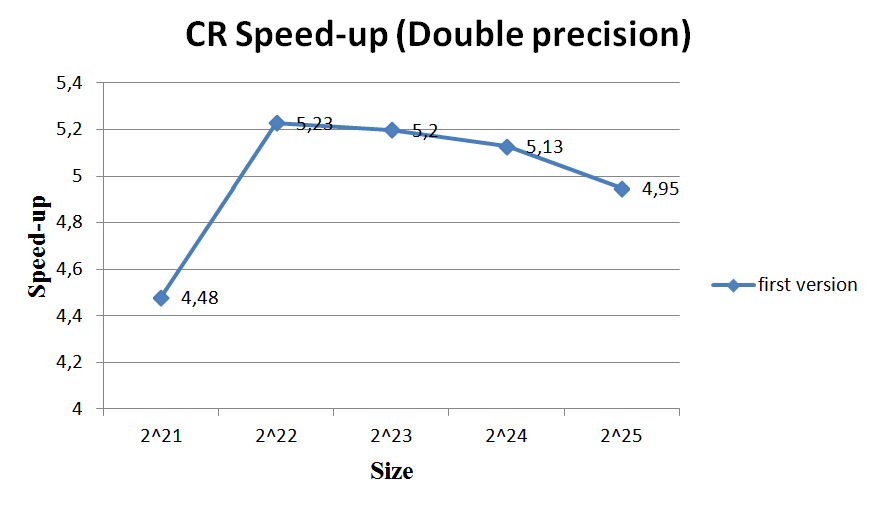
\includegraphics[width=1\textwidth]{grafhmata/cr_first_dp_speedup.png}
   \caption{Speedup Cyclic Reduction(DP)}
   \label{fig:Speedup Cyclic Reduction(DP)}
\end{figure}

\begin{table}[H]
\caption{Cyclic Reduction (padding version) execution time (DP)} 
\centering 
\begin{tabular}{| l | p{3cm} | p{3cm} |} 
\hline\hline 
Size & CPU & GPU  \\ [0.8ex] 
\hline 
        $2^{21}$ & $0.156$& $0.03$ \\ 	
        $2^{22}$ & $0.28$& $0.06$  \\ 	
        $2^{23}$ & $0.594$& $0.118$ \\ 
        $2^{24}$ & $1.09$& $0.237$ \\ 
        $2^{25}$ & $2.187$& $0.463$  \\ 
        $2^{26}$ & $--$& $--$      \\ [1ex]
\hline 
\end{tabular}
\label{table:cr_padding_double} 
\end{table}

\begin{table}[H]
\caption{Cyclic Reduction (padding version) speed - up (DP)} 
\centering 
\begin{tabular}{| l | p{3cm} |} 
\hline\hline 
size	 & Speed - up  \\  [0.8ex] 
\hline        
        $2^{21}$ & $5.2$      \\	
        $2^{22}$ & $4.66$     \\
        $2^{23}$ & $5.03$      \\ 
        $2^{24}$ & $4.59$    \\ 
        $2^{25}$ & $4.72$     \\ 
        $2^{26}$ & $--$       \\ [1ex]
        \hline
\end{tabular}
\label{table:cr_padding_double_spup} 
\end{table}


\newpage
    \begin{table}[H]
\caption{Block Cyclic Reduction N=3} 
\centering 
\begin{tabular}{| l |  p{1cm} |p{2,5cm}| p{2,5cm} |  p{2,5cm}| p{2,5cm} | } 
\hline\hline 
N & Q & CPU(parallel) & CPU(seq) & GPU(first)  & GPU(second)\\ [0.8ex] 
\hline
$3$ &	$127$ & $0.003$	&	$0.000$ & $0.010$ &  $0.005$ \\
$3$ &	$255$ & $0.013$	&	$0.010$ & $0.020$ & $0.018$ \\
$3$ &	$511$ & $0.065$	& $0.120$ & $0.050$ & $0.050$ \\
$3$ &	$1023$ & $0.328$	&	$0.820$ & $0.145$ & $0.168$ \\
$3$ &	$2047$ & $2.145$	&	$6.200$ & $0.403$ & $0.828$ \\
$3$ &	$4095$ & $17.363$	&	$47.700$ & $1.400$ & $4.365$ \\[1ex]
\hline 
\end{tabular}
\label{table:bcr_n=3} 
\end{table}

\begin{table}[H]
\caption{Block Cyclic Reduction N=7} 
\centering 
\begin{tabular}{| l |  p{1cm} |p{2,5cm}| p{2,5cm} |  p{2,5cm}| p{2,5cm} | } 
\hline\hline 
N & Q & CPU(parallel) & CPU(seq) & GPU(first)  & GPU(second) \\ [0.8ex] 
\hline
$7$ &	$127$ & $0.007$	&	$0.010$ & $0.010$ & $0.010$ \\
$7$ &	$255$ & $0.025$	&	$0.040$ & $0.035$ & $0.035$ \\
$7$ &	$511$ & $0.145$	&	$0.330$ & $0.120$ & $0.117$\\
$7$ &	$1023$ & $0.948$	&	$2.400$ & $0.425$ & $0.422$ \\
$7$ &	$2047$ & $6.697$	&	$18.020$ & $2.340$ & $2.325$ \\
$7$ &	$4095$ & $51.395$	&	$140.080$ & $10.857$ & $10.825$ \\[1ex]
\hline 
\end{tabular}
\label{table:bcr_n=7} 
\end{table}

   \begin{table}[H]
\caption{Block Cyclic Reduction N=15} 
\centering 
\begin{tabular}{| l |  p{1cm} |p{2,5cm}| p{2,5cm} |  p{2,5cm}| p{2,5cm}  |} 
\hline\hline 
N & Q & CPU(parallel) & CPU(seq) & GPU(first)  & GPU(second) \\ [0.8ex] 
\hline
$15$ &	$127$ & $0.013$	&	$0.020$ & $0.025$ & $0.022$ \\
$15$ &	$255$ & $0.058$	&	$0.110$ & $0.070$ & $0.075$ \\
$15$ &	$511$ & $0.320$	&	$0.800$ & $0.268$ & $0.268$ \\
$15$ &	$1023$ & $2.272$	& $5.870$  & $0.993$ & $0.985$ \\
$15$ &	$2047$ & $17.385$	&	$44.470$ & $5.300$ & $5.287$ \\
$15$ &  $4095$ & $126.210$	&	$347.420$ & $25.312$ &  $25.383$\\[1ex]
\hline 
\end{tabular}
\label{table:bcr_n=15} 
\end{table}

   \begin{table}[H]
\caption{Block Cyclic Reduction N=31} 
\centering 
\begin{tabular}{| l |  p{1cm} |p{2,5cm}| p{2,5cm} |  p{2,5cm}| p{2,5cm} | } 
\hline\hline 
N & Q & CPU(parallel) & CPU(seq) & GPU(first)  & GPU(second) \\ [0.8ex] 
\hline
$31$ &	$127$ & $0.025$	&	$0.040$ & $0.040$ & $0.045$ \\
$31$ &	$255$ & $0.115$	&	$0.240$ & $0.152$ & $0.150$ \\
$31$ &	$511$ & $0.685$	&	$1.760$ & $0.568$ & $0.568$ \\
$31$ &	$1023$ & $5.160$	& $13.110$ & $2.150$ & $2.147$ \\
$31$ &	$2047$ & $32.672$	& $99.650$  & $10.867$ & $10.852$ \\
$31$ &	$4095$ & $243.312$	& $783.830$ & $--$ & $54.682$ \\ [1ex]
\hline 
\end{tabular}
\label{table:bcr_n=31} 
\end{table}

   \begin{table}[H]
\caption{Block Cyclic Reduction N=63} 
\centering 
\begin{tabular}{| l |  p{1cm} |p{2,5cm}| p{2,5cm} |  p{2,5cm}| p{2,5cm} |} 
\hline\hline 
N & Q & CPU(parallel) & CPU(seq) & GPU(first)  & GPU(second)\\ [0.8ex] 
\hline

$63$ &	$127$ & $0.050$	&	$0.080$ & $0.085$ & $0.087$ \\
$63$ &	$255$ & $0.235$	&	$0.510$ & $0.305$ & $0.307$ \\
$63$ &	$511$ & $1.393$	&	$3.700$ & $1.167$ & $1.173$\\
$63$ &	$1023$ & $10.582$	& $27.990$ & $4.503$ & $4.468$ \\
$63$ &	$2047$ & $70.007$	& $213.560$ & $22.192$ & $22.105$ \\
$63$ &	$4095$ & $611.175$	& $1677.440$ & $--$ & $112.907$ \\[1ex]
\hline 
\end{tabular}
\label{table:bcr_n=63} 
\end{table}

   \begin{table}[H]
\caption{Block Cyclic Reduction N=127} 
\centering 
\begin{tabular}{| l |  p{1cm} |p{2,5cm}| p{2,5cm} |  p{2,5cm}| p{2,5cm} | } 
\hline\hline 
N & Q & CPU(parallel) & CPU(seq) & GPU(first)  & GPU(second) \\ [0.8ex] 
\hline
$127$ &	$255$ & $0.475$	&	$1.040$ &	$0.620$ & $0.625$ \\
$127$ &	$511$ & $2.835$	&	$7.630$ & 	$2.382$ & $2.393$ \\
$127$ &	$1023$ & $21.898$	& $58.090$ & 	$8.893$ & $8.875$ \\
$127$ &	$2047$ & $149.167$	& $444.920$ & 	$43.877$ & $43.765$ \\
$127$ &	$4095$ & $1248.453$	& $3493.550$ & 	$--$ & $231.595$ \\[1ex]
\hline 
\end{tabular}
\label{table:bcr_n=127} 
\end{table}

\begin{figure}[H]
   \centering
       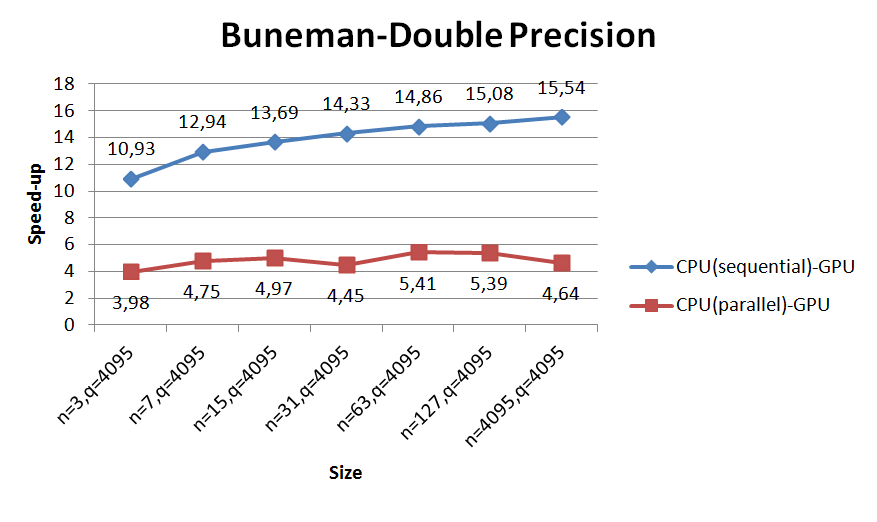
\includegraphics[width=1\textwidth]{grafhmata/buneman_dp_speedup.png}
   \caption{Speedup Buneman(DP)}
   \label{fig:Speedup Buneman(DP)}
\end{figure}

   \begin{table}[H]
\caption{Block Cyclic Reduction N=Q} 
\centering 
\begin{tabular}{| l |  p{1cm} |p{2,5cm}| p{2,5cm} |  p{2,5cm}| p{2,5cm} | } 
\hline\hline 
N & Q & CPU(parallel) & CPU(seq) & GPU(first)  & GPU(second)\\ [0.8ex] 
\hline
$127$ &	$127$ & $0.100$	&	$0.160$ & $0.170$ & $0.170$ \\
$255$ &	$255$ & $0.960$	&	$2.120$ & $1.250$ & $1.262$ \\
$511$ &	$511$ & $11.355$	&	$31.340$ & $9.640$ & $9.697$ \\
$1023$ &	$1023$ & $169.595$	&	$482.900$ & $65.748$ & $65.790$ \\
$2047$ &	$2047$ & $,$	&	$7437.090$ & $694.060$ & $692.940$ \\
$4095$ & $4095$  & $,$	&  $117200.020$ & $--$ & $7542.910$ \\[1ex]
\hline 
\end{tabular}
\label{table:bcr_n=q} 
\end{table} 

\begin{figure}[H]
   \centering
       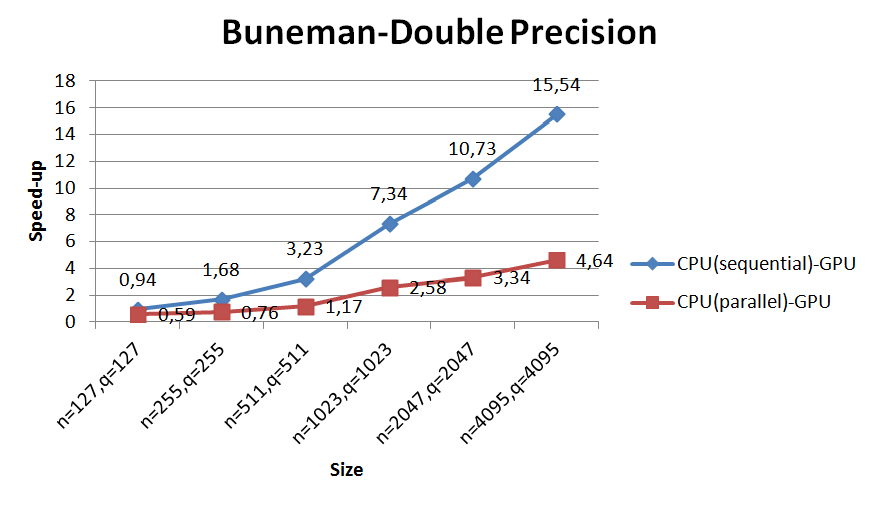
\includegraphics[width=1\textwidth]{grafhmata/buneman_dp_speedup_nq.png}
   \caption{Speedup Buneman N=Q (DP)}
   \label{fig:Speedup Buneman N=Q (DP)}
\end{figure}
The same observations with the single precision apply here. In the case of cyclic reduction algorithm the speed - up decrease starts in smaller size due to almost double memory transfers. Likewise, padding does not effect performance.
 A smaller but equally remarkable speed - up up to 15x was achieved in Block cyclic reduction when ported to GPU. Again the memory transfers now are almost twice therefore consume more significant portion of the total execution time.
\subsection{Conclusions}
Solving PDEs in one dimension and two dimensions demands intensive computation load in both time and space.
Due to wide appliance of PDEs in many scientific fields a need for speeding the computation arised. The GPGPU
wave came with the solution to this.
Particularly, after a deep search in the effort made in this area we conclude that cyclic reduction algorithm 
was the most efficient to perform on GPUs. Also it is remarkable that very few implementations of block cyclic reduction on GPUs  exist and none in our knowledge of Buneman variant.\\
In cyclic reduction algorithm up to 8x speedup was observed in single precision and up to 5x in double precision.
After a certain size speed-up started to decrease due to large memory transfers. Padding technique was applied with
no performance impact.\\
In Buneman algorithm up to 25x speedup was observed in single precision and up to 15x in double precision in single
threaded CPU and up 8.5x to in single precision and up to 5.5x in double precision. Several optimizations were applied. MKL and Lapack libraries were used for CPU programming and CUBlas and CULapack were used for the GPU programming.In the CPU implementation both sequential and multi- threaded versions were made. A sliding window technique was used in order to increase the problem size. An attempt to overlap computations with memory tranfers using streams was made with no performance impact.\\
In both algorithms single precision outperforms double precision since in the second approximately twofold memory 
tranfers occurred.\\
Conclusively, it was proven that solving PDEs in both one and two dimensions on GPUs can give significant performance
in relation to CPU implementation. 
\subsection{Further Improvements}
As referred in previous sections both algorithms were tested using the Poisson differential equation 
as a model. However, the implementations were implemented in a way to be easily expanded in order to model 
several mathematical and physical problems.  
As a case study we plan to apply the Buneman method to a reaction-diffusion PDE.  This PDE is considered as a common simplified model for studying the expansion of gliomata in the human brain. This would lead to adapt time as a parameter in the calculation process. Buneman algorithm will be called repeatably in a loop, which will calculate the
PDE's coefficients in every time step.